\documentclass[12pt]{article}

\usepackage{sbc-template}

\usepackage{graphicx,url}

\usepackage[english]{babel}   

\usepackage[utf8]{inputenc}  
% UTF-8 encoding is recommended by ShareLaTex

\usepackage{listings}

\usepackage{float}

\sloppy

\title{Authentication of Identity Documents Using DNSSEC, Digital Signatures and QR Codes}

\author{Luiz Fernando Ribeiro Amaral\inst{1},\\ 
Jorge Guilherme Silva dos Santos\inst{1}, Mateus Almeida Rocha\inst{1}, \\ 
Joseph Gersch\inst{2}, Georges Daniel Amvame-Nze\inst{1},\\ 
Robson de Oliveira Albuquerque\inst{1}, Rafael Timóteo de Sousa Júnior\inst{1}}


\address{Decision Technologies Laboratory - LATITUDE\\Electrical Engineering Department\\University of Brasília (UnB)\\
Brasília, DF, Brazil
\nextinstitute 
Department of Computer Science\\Colorado State University\\Fort Collins, CO, USA 
\email{\{luiz,jorge,mateus,robson\}@redes.unb.br,}
\email{jgersch@colostate.edu,} 
\email{\{georges,desousa\}@unb.br}
 }

\begin{document} 

\lstset{
	%basicstyle=\ttfamily,
	basicstyle=\ttfamily\scriptsize,
	%keywordstyle=\color{blue},
	%stringstyle=\color{green},
	%commentstyle=\color{red},
	keywordstyle={},
	stringstyle={},
	commentstyle={},
	showspaces=false,
	showstringspaces=false,
	breaklines=true,
	breakautoindent=true,
	captionpos=b,
	xleftmargin=0pt,
	framexleftmargin=4pt,
	breaklines = true,
	extendedchars=true,
	inputencoding=utf8,
	numbers=none,
	mathescape=false,
% 	backgroundcolor=\color{light-gray},
	frame=none
}

\maketitle

\begin{abstract}
  This paper describes a system for authenticating identity documents by digitally signing the data and embedding it in a 2D code to be printed with the document. In the proposed scheme, a message is digitally signed using a digital signature block which is stored in a QR Code. The code is later scanned by the user and, after validation, the corresponding digital information can be compared with the printed information. The authenticity of the message is guaranteed using RSA digital signatures and a secure DNS implementation based on DANE and DNSSEC for the certificate distribution. A proof of concept was implemented using the ISC BIND DNS Server and OpenSSL to create and distribute the certificates and a Telegram Bot for signature verification.
\end{abstract}
     
\section{Introduction}

Document counterfeiting is on the rise as sophisticated printing and scanning technologies become cheap, enabling criminals to take advantage of digital technology to produce high quality fraudulent documents. Society relies on experts for verifying the authenticity of these documents using special tools and document properties, an almost impossible job for entities dealing with thousands of documents daily \cite{garain2008automatic}. 

The system proposed in this paper addresses the verification of an identity document by enabling any person to verify the information contained in this document using a smartphone application. There is no need for specialized people or physical security features in the document itself. 

Compared to previous work \cite{warasart2012based}, this system does not rely on a certificate authority to provide valid certificates, nor does it need to have the certificates preloaded by the application used for signature validation. Using DNSSEC (Domain Name System Security Extensions) enabled servers, the certificates can be published in the signing entity zone and the authenticity and integrity of the data can be guaranteed by the chain of trust provided by DNSSEC signatures \cite{arends2005dns}. 

Digital signatures are a standard for guaranteeing authenticity and integrity nowadays. \emph{A digital signature algorithm allows an entity to authenticate the integrity of signed data and the identity of the signatory. The recipient of a signed message can use a digital
signature as evidence in demonstrating to a third party that the signature was, in fact, generated by the claimed signatory} \cite{fips2013186}. In our proposed scheme, a message is digitally signed using a digital signature block which is stored in a QR Code which is printed on the identity document, such as for instance a driver's license containing a QR Code with the message and its signature as shown in Figure \ref{fig:license}.

\begin{figure}[ht]
    \centering
    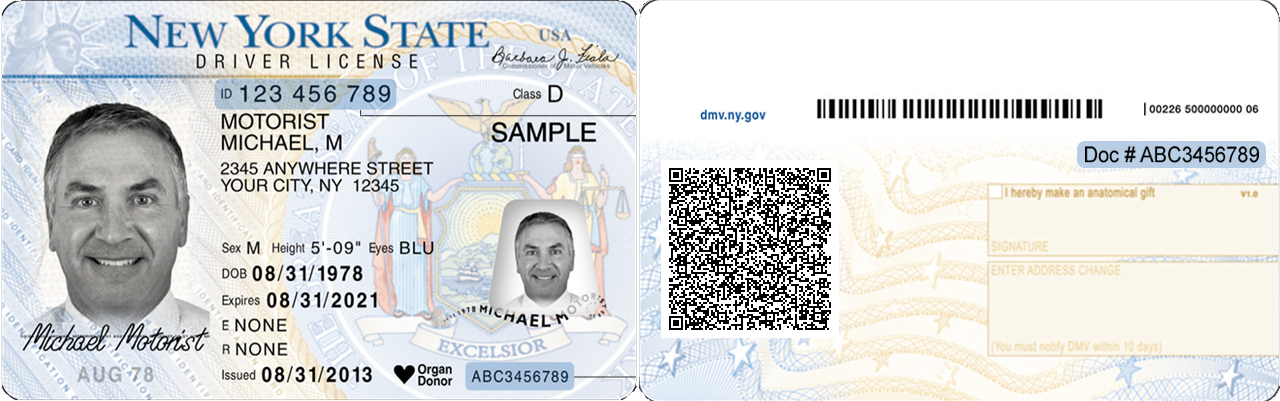
\includegraphics[width=1\textwidth]{license.png}
    \caption{Driver's license example. Adapted from \cite{new_sample_2013}}
    \label{fig:license}
\end{figure}

This paper is organized so the complete system architecture is first described and then a proof of concept implementation of the system is presented.

\section{The System Architecture}

The architecture is composed of signing entities, which can be governmental institutions or companies who issue identification documents, a phone application used for the signature validation and the DNS infrastructure. Figure \ref{fig:overview} shows a complete diagram of the system. Each entity can have a signing server, for storing the keys and generating the QR Codes with the signatures and the DNS servers to provide the certificates for signature validation. A user, using his smartphone scans the QR Code using the camera. The phone decodes the data and queries the DNS server to retrieve the certificate and validate the DNSSEC chain of trust. It then validates the signature using the retrieved certificate and if valid, presents the data to the user.

\begin{figure}[ht]
    \centering
    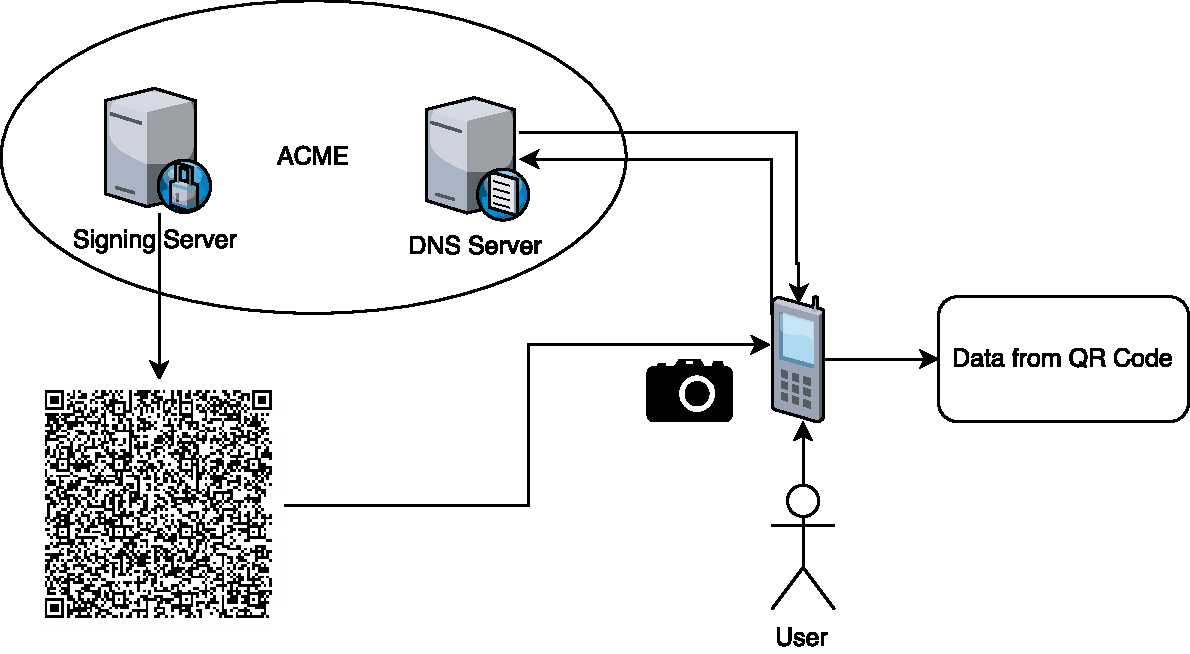
\includegraphics[width=0.8\textwidth]{overview.pdf}
    \caption{System Architecture Overview[Source: Authors]}
    \label{fig:overview}
\end{figure}

A key feature is that, while other implementations propose the use of optical character recognition (OCR) for obtaining the message for validation \cite{warasart2012based}, we rely on a person to validate the document by comparing digitally signed data contained in the QR Code message with the actual data printed on the document.

\subsection{DNS Servers}

Although the CERT Resource Record specification allows the storage of certificates in insecure DNS zones, it specifies that in these cases the whole certificate chain needs to be validated, exacerbating the principle of relying on a certificate authority. To be able to trust the certificate without the need of verifying the whole certificate chain, we propose the use of CERT or DANE self-signed certificates in the DNS. In this case, the zone must be secure, i.e, DNSSEC-enabled, and the record authenticity verified by using DNSSEC \cite{josefsson2006storing}. 

The DNSSEC specification defines the required behavior for DNSSEC-enabled zones, including serving keys, signatures, secure denial of existence and serving the zone securely in all of the authoritative name servers \cite{osterweil2009deploying}.  NIST allows the use of 1024-bit RSA keys for DNSSEC, as long as other key management practices are put in place, to avoid key compromise \cite{chandramouli2013secure}.

\subsection{Message Format}

The messages used by the system consist of JSON objects such as shown in Figure \ref{fig:json}. JSON is a lightweight, text-based, language-independent data interchange format \cite{bray2014javascript}. This choice brings flexibility to the data format, making it easy to add or remove fields, without the need to completely rewrite data templates or the application itself.

\begin{figure}[ht]
    \centering
    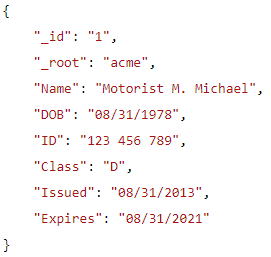
\includegraphics[width=0.4\textwidth]{json.png}
    \caption{Example Message [Source: Authors]}
    \label{fig:json}
\end{figure}

The message object needs two mandatory values: \textit{\_root} and \textit{\_key}, representing the DNS root and the key identifier, respectively. These fields indicate where to find the certificate needed for signature validation. The validating application still needs to know the DNS zone corresponding to the indicated \textit{\_root} to fetch the certificate, but the key field brings more flexibility, as the signing entity can easily add more certificates to the DNS infrastructure without the need of updating the signature validation application. 

\subsection{Information Signing}

The message is signed using the RSA digital signature scheme, with 2048-bit RSA private keys, the SHA-512 hash algorithm and the PSS padding scheme, meeting the recommendations established by NIST in the SP800-57 Part 3 Rev. 1 \cite{nist800}.

Figure \ref{fig:signature} illustrates the message signature process. The issuer of a document calculates the message SHA-512 hash, encrypts it using the RSA private key and finally appends it to the end of the message. Message and signature are then published in the form of a QR Code on the printed document. It is valid mentioning that the padding and mask generation operations were removed from the figure for simplicity.

\begin{figure}[ht]
    \centering
    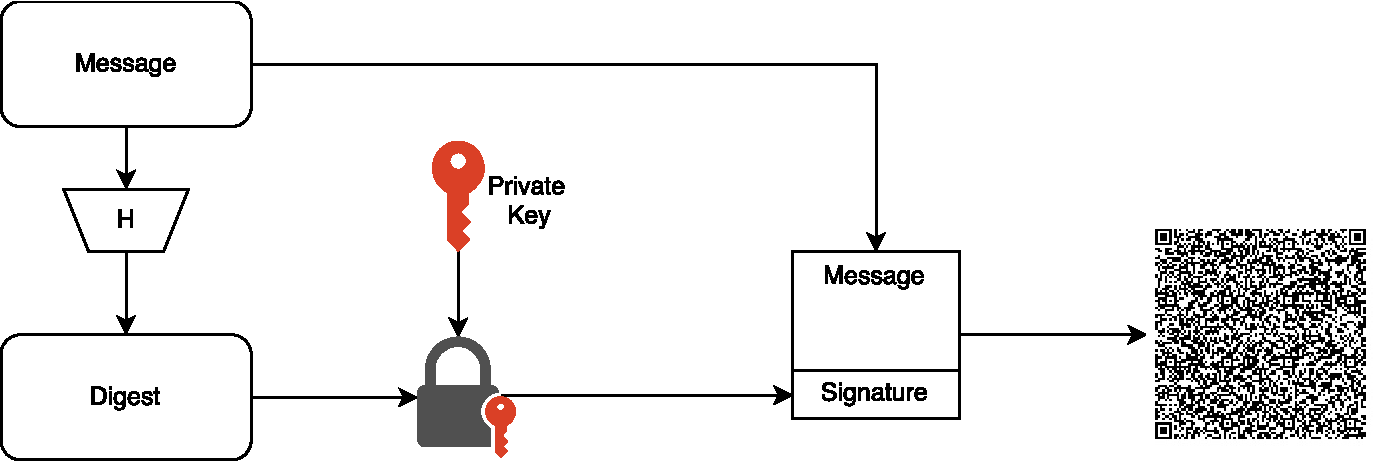
\includegraphics[width=.8\textwidth]{signing.pdf}
    \caption{Message signature process. [Source: Authors]}
    \label{fig:signature}
\end{figure}

\subsection{QR Code}

A QR Code is one of the many kinds of 2D codes. It was invented in 1994 to be used in automotive industry and became an ISO standard in 2000. Nowadays it has become widespread, being used in electronic components labeling, aircraft and space industrial data-product identification, bus tickets, betting tickets, patient identification in hospitals and many other applications in all kinds of fields \cite{soon2008qr}.

The QR Code specification states that it can store 2,953 characters at maximum when using 8-bit binary mode. Other modes are available and offer higher capacity, but are limited and don't cover our use case. Table \ref{tab:capacity} shows the capacity of each of the available modes.

\begin{table}[ht]
\centering
\caption{QR Code capacity for each mode. Adapted from \cite{soon2008qr}}
\label{tab:capacity}
\begin{tabular}{|c|c|}
\hline
\textbf{Mode}        & \textbf{Capacity}           \\ \hline
Numerical characters & 7,089 characters at maximum \\ \hline
Alphanumerical       & 4,296 characters at maximum \\ \hline
Binary (8 bit)       & 2,953 characters at maximum \\ \hline
Kanji characters     & 1,817 characters at maximum \\ \hline
\end{tabular}
\end{table}

The QR Code standard states that the alphanumeric mode, for example, covers only part of the ASCII character table and doesn't include the brackets and colon (\{,\},:) used in the JSON message object. One way to make our data comply with the requirements of the alphanumeric mode would be encoding it using Base32, but the gain in data capacity between the alphanumeric mode and the binary mode is approximately 45\%, while the Base32 encoding adds an overhead of 60\%, making it inefficient for use with the alphanumeric mode \cite{josefsson2006base16}. 
Our proposed system is designed for the authentication of identity documents, which usually don't carry a large amount of data. For example, a drivers license contains an ID number, name, address, sex, height, DOB, expiration date and issuance date. In the case of an application that needs to carry a big amount of data, compression may be applied to the data and signature which will help to reduce the size of the QR Code printout. 

\subsection{Storing Certificates on the DNS}

The certificates used for signature validation are stored in the signing entity DNS zone under CERT Resource Records. According to \cite{josefsson2006storing}, \emph{it is recommended that certificate CERT Resource Records be stored under a domain name related to their subject, i.e., the name of the entity intended to control the private key corresponding to the public key being certified}. Hence, each document issuer who uses the system will store its certificates under its own DNS domain name and zone. 

The structure of a CERT Resource Record is shown in Figure \ref{fig:certrr}. in this structure, the certificate type field defines the type of data contained in the record. In our case, this field is set with type 1 - PKIX. The key tag field is a 16-bit value computed from the certificate public key used for efficient public key selection. The algorithm used for computation is specified in \cite{arends2008rfc}, Appendix B. The algorithm field identifies the digest algorithm used. This value changes based on the certificate being published in the record and a full list of algorithms and their IDs can be found in \cite{iana_domain_2017}. Finally, the Base64 encoded certificate goes into the certificate field.

\begin{figure}[ht]
    \centering
    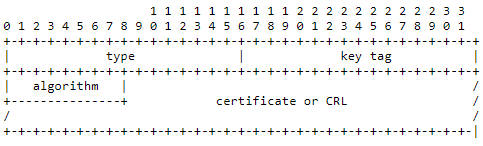
\includegraphics[width=.8\textwidth]{certrr.png}
    \caption{CERT Resource Record Structure (Numbers on top indicate each bit). Source: \cite{josefsson2006storing}.}
    \label{fig:certrr}
\end{figure}

\subsection{Signature Validation}

This process, as shown in Figure \ref{fig:verification}, is performed in a smartphone, beginning with the QR Code capture by the device camera. After scanning the QR Code, the signature validation is quickly done, as the process of decryption only takes milliseconds in most contemporary smartphones \cite{thiranant2015performance}. 

\begin{figure}[ht]
    \centering
    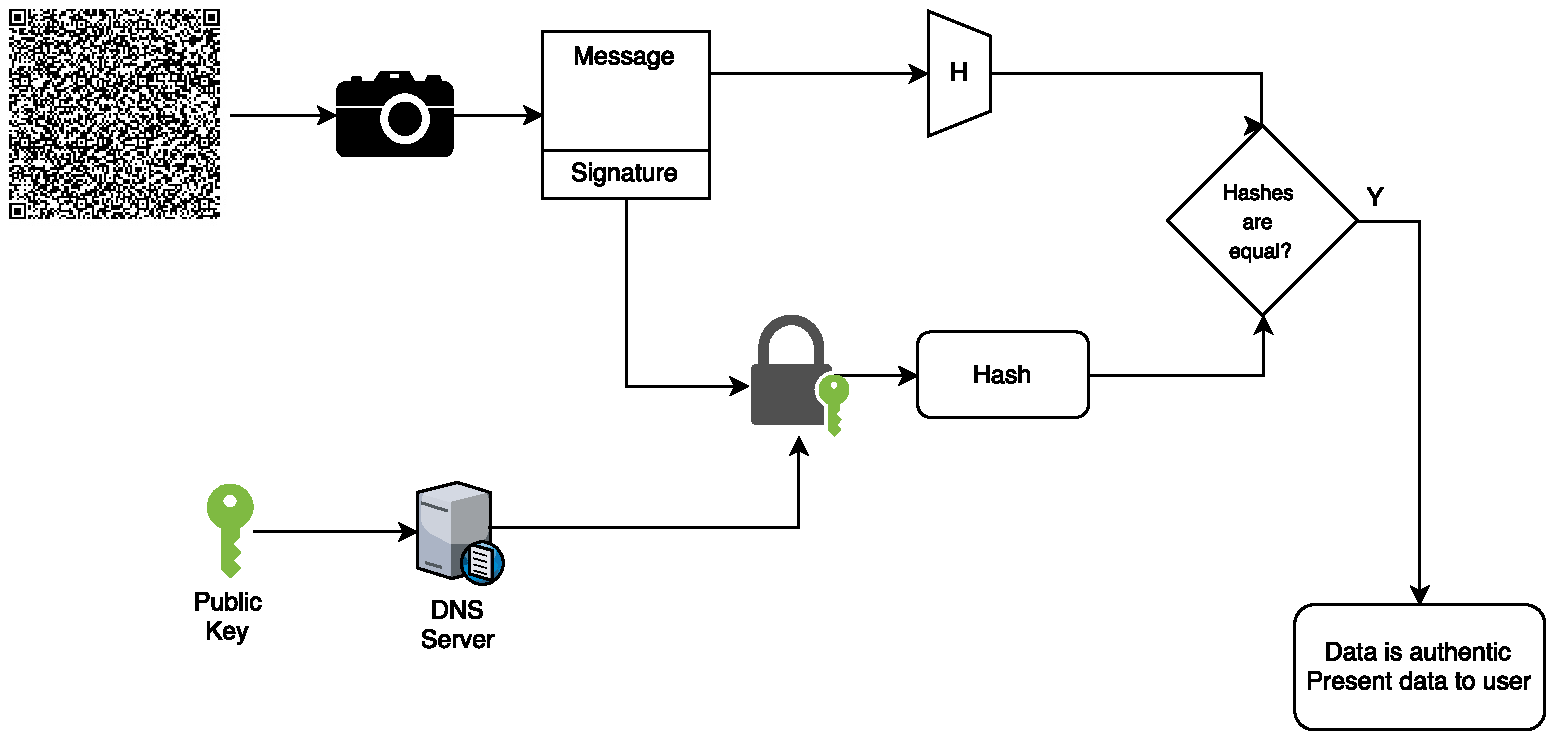
\includegraphics[width=.8\textwidth]{verification.pdf}
    \caption{Signature validation process [Source: Authors]}
    \label{fig:verification}
\end{figure}

Thus, to validate the signature, the user takes a picture of the identification document QR Code using a smartphone. The application then splits the message and signature and starts two different processes. The first one calculates the SHA-512 hash of the message and keep it for later usage. The second process uses the \textit{\_root} and \textit{\_key} contained in the message to fetch the certificate from the DNS server and then decrypts the signature data and obtains the hash of the signed message. By comparing the two hashes, the authenticity of the message contained in the QR Code can be guaranteed. 

The validation process in Figure \ref{fig:verification} authenticates the message contained in the QR Code, but does not guarantee that the data in the printed document is authentic. This second validation needs to be done by the user, by visual comparison between the data presented by the application and the data in the document. 

\section{Proof of Concept}

To evaluate the proposed architecture, a proof of concept was implemented using open-source software tools. A certificate authority was created using OpenSSL, two ISC BIND DNS servers were setup in master-slave operation, a web API was created to execute the signature operation and a Telegram Bot was used to provide an user interface for signature verification. 

\subsection{Certificate Authority}

Using the default OpenSSL settings, an example certificate authority was created and two certificates, for two example companies were issued. The private keys related to the certificates were 2048-bit long, as recommended by NIST. 

\subsection{DNS Zone}

To achieve the stated requirements, the system was implemented using two DNS servers, one master and one slave. Two example zones, representing pseudo-organizations Acme and Globex, respectively acme.luiz.eng.br and globex.luiz.eng.br, were created to hold the certificates used for the signatures. The zones were implemented with DNSSEC, in a pre-existing DNSSEC-enabled infrastructure. 

While the acme.luiz.eng.br zone has a valid DNSSEC signature and valid DS entries in the parent zone, the zone globex.luiz.eng.br only has the DS entries in the parent zone, resulting in a signature validation failure as the zone is in a bogus state, simulating for example, a cache poisoning situation. 

To verify the secure status of the ACME zone and bogus status of the Globex zone, we used the Verisign DNSSEC Analyzer \cite{verisign_dnssec}. Figure \ref{fig:dnssecvalid} shows the result of the DNSSEC validation for both zones, where the Globex zone does not contain a DNSKEY record, neither RRSIGs.

\begin{figure}[H]
    \centering
    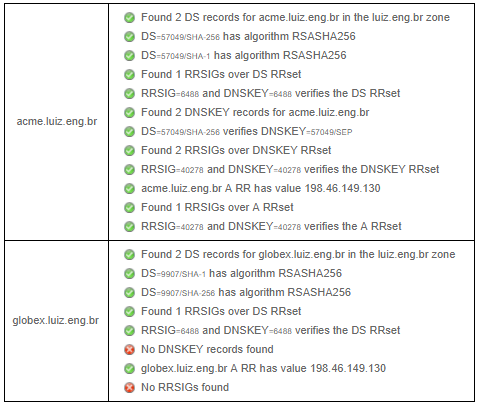
\includegraphics[width=0.8\textwidth]{dnssecvalid.png}
    \caption{DNSSEC validation of the zones. Adapted from \cite{verisign_dnssec}}
    \label{fig:dnssecvalid}
\end{figure}

After setting up the zone, the certificates were published following the RFC4398 \cite{josefsson2006storing} specification, except for the naming scheme, as it is just a recommendation. The first certificate, the one for the fictitious Acme organization, was published under 1.acme.luiz.eng.br, and the second, for the fictitious Globex Corporation, was published under 1.globex.luiz.eng.br. 

\subsection{Message Signing}

In our implementation, we used the Tornado Web Framework \cite{python_tornadoweb} to implement a Web API for message signing. With this API, two messages were signed to be used later in the validation process. The messages are JSON objects containing sample data of a driver's license, as shown in Figure \ref{fig:json}. A sample output from the API can be seen in Figure \ref{fig:api}.

\begin{figure}[H]
    \centering
    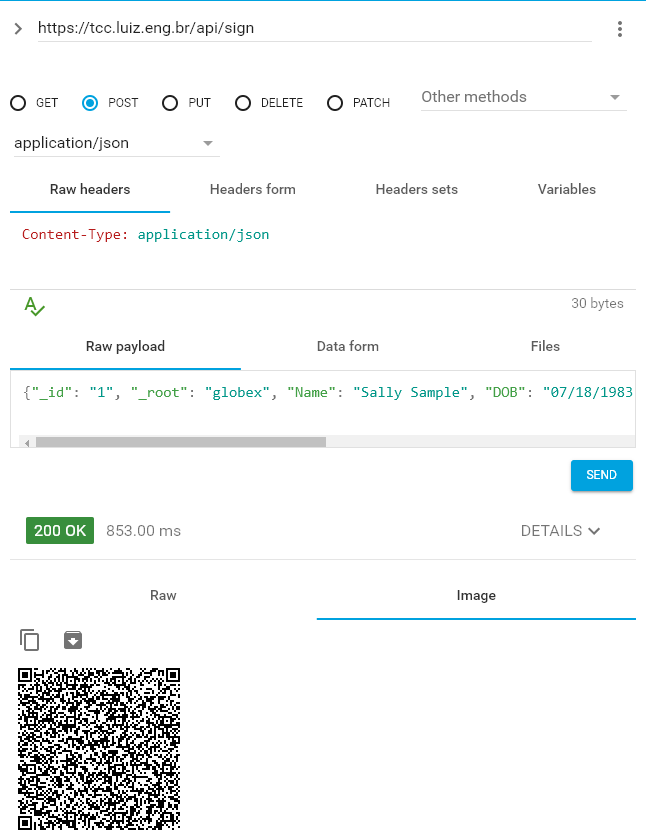
\includegraphics[width=0.8\textwidth]{api.png}
    \caption{API Signature Request [Source: Authors]}
    \label{fig:api}
\end{figure}

The message signing itself is implemented through the hazardous materials layer of the Python Cryptography \cite{python_cryptography} package. The hazardous materials layer contains low-level cryptography primitives, meaning that the functions included with it should be used carefully, as they can result in an insecure implementation.

The binary output of the signature function is encoded in Base64, so we can later separate the message from its signature using the ASCII character 0x1F, without the risk of having this same byte in the signature data.

When using a 2048-bit key, the produced signature is 256 bytes long and after the Base64 encoding, which has a 4:3 ratio \cite{josefsson2006base16}, will result in a 344 bytes long string, leaving room for up to 2609 bytes for the message, although the utilization of this data depends on the QR Code capacity.

Despite all the capacity left for the message, a QR Code to store all this data, would be too big to fit on an identity document. A solution is to employ the feature of QR Code linking, allowing the division into symbols enabling the printing even if there is not enough space available for the complete QR Code. Figure \ref{fig:linking} shows an example of the linking technique.

\begin{figure}[H]
    \centering
    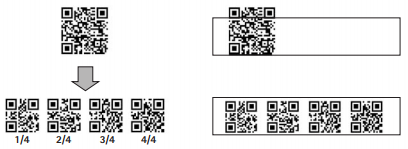
\includegraphics{linking.png}
    \caption{An example of QR Code linking \cite{soon2008qr}}
    \label{fig:linking}
\end{figure}

Regarding the example message in Figure \ref{fig:json}, which has only 154 bytes and is small enough for its resulting QR Code to fit in an identity document, as the example shown in Figure \ref{fig:license}, the QR Code linking feature was not employed in our proof of concept. 

To prove that the system works, two different messages were signed and a QR Code was created for each of them. The two created QR Codes can be seen in Figures \ref{fig:qrcode1} and \ref{fig:qrcode2}.

\begin{figure}[H]
    \centering
    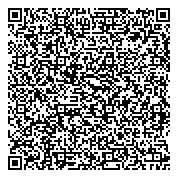
\includegraphics[width=0.3\textwidth]{qrcode1.png}
    \caption{QR Code containing the message with a valid signature [Source: Authors]}
    \label{fig:qrcode1}
\end{figure}

\begin{figure}[H]
    \centering
    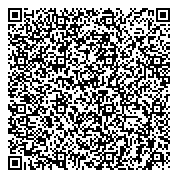
\includegraphics[width=0.3\textwidth]{qrcode2.png}
    \caption{QR Code containing the message with an invalid signature [Source: Authors]}
    \label{fig:qrcode2}
\end{figure}

\subsection{Signature Validation}

The signature validation is done through a Telegram Bot \cite{telegram_bot}, as we considered it a simple way to implement a nice mobile user interface using Python. This decision makes our solutions multi-platform, so that the users can interact with the Bot using the Telegram app on different devices, including iPhones and Android phones.

To validate the signature, the Telegram Bot decodes the QR Code and splits the resulting data into message and encoded signature, considering the 0x1F character as their separator. The Bot then maps the \textit{\_root} field of the message to a list of zones already known to it and uses the \textit{\_key} field to build the complete DNS name to fetch the certificate. 

When fetching the certificate, the validity of the DNSSEC signatures is checked, to establish if the returned data can be trusted or not. If the returned response has an invalid DNSSEC signature or no DNSSEC at all, the certificate cannot be trusted and, by consequence, the signature will be considered invalid. 

If the certificate fetching is successful, the message is validated against the signature and, if the data matches, the information contained in the message is presented to the user. Figure \ref{fig:result} shows the resulting output for the two example QR Codes mentioned before. 

\begin{figure}[ht]
    \centering
    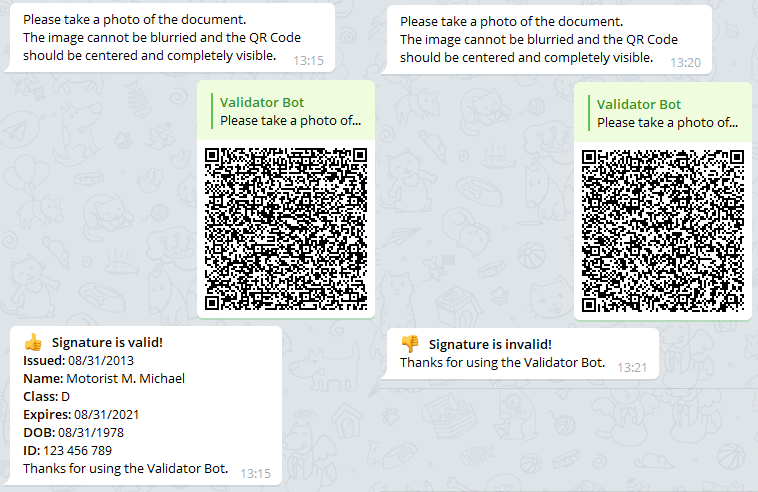
\includegraphics[height=0.38\textheight]{result.png}
    \caption{Bot messages after validating the two signatures [Source: Authors]}
    \label{fig:result}
\end{figure}

\section{Conclusion and Future Work}

The proposed architecture can provide a distributed, flexible yet safe way of guaranteeing the authenticity of identity documents without the need of relying completely on a trusted third-party. By using the DNS infrastructure for certificate retrieval, identity document issuers can create and manage their own keys, making it easier to execute key rollovers for example, as the keys don't need to be preloaded by the verifying application or party.

The decentralization of the keys makes it harder for an attacker to compromise the whole system. As the keys are distributed, an attacker would have to breach into each of the subsystems to acquire all the keys and the DNSSEC guarantees that the keys stored on the DNS are served in a secure manner, preventing attacks like cache poisoning and alteration of the keys stored in the zone. By means of DANE, we are able to use and trust self-signed certificates, removing the need of a Public Key Infrastructure and reducing the costs related to a third-party Certificate Authority.

In the future, optical character recognition techniques can be used to automate the validation of identity documents, removing the need of a visual comparison done by the user. The security can be increased by including a timestamp to prevent replay attacks and including a serial number to provide an identifier to enable traceability by the issuer.

\section*{Acknowledgments}
This research work has the support of the Brazilian research and innovation Agencies CAPES – Coordination for the Improvement of Higher Education Personnel (Grant 23038.007604/2014-69 FORTE – Tempestive Forensics Project) and CNPq – National Council for Scientific and Technological Development (Grant 465741/2014-2 Science and Technology National Institute – INCT on Cyber Security), as well as the Brazilian Ministry of Planning, Development and Management (Grants 005/2016 DIPLA – Planning and Management Directorate, and 11/2016 SEST – State-owned Federal Companies Secretariat), as well as Secure64 Software Corporation, for technical information on DNSSEC deployment and behavior.


\bibliographystyle{sbc}
\bibliography{sbc-template}

\end{document}
